\documentclass[10pt, a5paper]{article}
\usepackage{pdfpages}
\usepackage{parallel}
\usepackage[T2A]{fontenc}
\usepackage{ucs}
\usepackage[utf8x]{inputenc}
\usepackage[polish,english,russian]{babel}
\usepackage{hyperref}
\usepackage{rotating}
\usepackage[inner=2cm,top=1.8cm,outer=2cm,bottom=2.3cm,nohead]{geometry}
\usepackage{listings}
\usepackage{graphicx}
\usepackage{wrapfig}
\usepackage{longtable}
\usepackage{indentfirst}
\usepackage{array}
\newcolumntype{P}[1]{>{\raggedright\arraybackslash}p{#1}}
\frenchspacing
\usepackage{fixltx2e} %text sub- and superscripts
\usepackage{icomma} % коскі ў матэматычным рэжыме
\PreloadUnicodePage{4}

\newcommand{\longpage}{\enlargethispage{\baselineskip}}
\newcommand{\shortpage}{\enlargethispage{-\baselineskip}}

\def\switchlang#1{\expandafter\csname switchlang#1\endcsname}
\def\switchlangbe{
\let\saverefname=\refname%
\def\refname{Літаратура}%
\def\figurename{Іл.}%
}
\def\switchlangen{
\let\saverefname=\refname%
\def\refname{References}%
\def\figurename{Fig.}%
}
\def\switchlangru{
\let\saverefname=\refname%
\let\savefigurename=\figurename%
\def\refname{Литература}%
\def\figurename{Рис.}%
}

\hyphenation{admi-ni-stra-tive}
\hyphenation{ex-pe-ri-ence}
\hyphenation{fle-xi-bi-li-ty}
\hyphenation{Py-thon}
\hyphenation{ma-the-ma-ti-cal}
\hyphenation{re-ported}
\hyphenation{imp-le-menta-tions}
\hyphenation{pro-vides}
\hyphenation{en-gi-neering}
\hyphenation{com-pa-ti-bi-li-ty}
\hyphenation{im-pos-sible}
\hyphenation{desk-top}
\hyphenation{elec-tro-nic}
\hyphenation{com-pa-ny}
\hyphenation{de-ve-lop-ment}
\hyphenation{de-ve-loping}
\hyphenation{de-ve-lop}
\hyphenation{da-ta-ba-se}
\hyphenation{plat-forms}
\hyphenation{or-ga-ni-za-tion}
\hyphenation{pro-gramming}
\hyphenation{in-stru-ments}
\hyphenation{Li-nux}
\hyphenation{sour-ce}
\hyphenation{en-vi-ron-ment}
\hyphenation{Te-le-pathy}
\hyphenation{Li-nux-ov-ka}
\hyphenation{Open-BSD}
\hyphenation{Free-BSD}
\hyphenation{men-ti-on-ed}
\hyphenation{app-li-ca-tion}

\def\progref!#1!{\texttt{#1}}
\renewcommand{\arraystretch}{2} %Іначай формулы ў матрыцы зліпаюцца з лініямі
\usepackage{array}

\def\interview #1 (#2), #3, #4, #5\par{

\section[#1, #3, #4]{#1 -- #3, #4}
\def\qname{LVEE}
\def\aname{#1}
\def\q ##1\par{{\noindent \bf \qname: ##1 }\par}
\def\a{{\noindent \bf \aname: } \def\qname{L}\def\aname{#2}}
}

\def\interview* #1 (#2), #3, #4, #5\par{

\section*{#1\\{\small\rm #3, #4. #5}}

\def\qname{LVEE}
\def\aname{#1}
\def\q ##1\par{{\noindent \bf \qname: ##1 }\par}
\def\a{{\noindent \bf \aname: } \def\qname{L}\def\aname{#2}}
}

\begin{document}
\title{Сравнение Redis и MySQL на задаче построения игровых рейтингов}
\author{Алексей Романов \footnote{Minsk, Belarus; {\tt drednout.by@gmail.com}}}
\maketitle
\begin{abstract}
During development of games often exists the problem of choosing the right tool for storing and processing data. In this paper MySQL and Redis are compared. The main technique of comparison is implementing the part of functionality using each of tool and analysing of obtained solution. The analysis includes both static code and data verification, and also real experiments with measuring all interesting parameters. Then experiment's data are processed and given results are  objectively compared.
\end{abstract}
В процессе разработки игр часто возникает задача построения рейтингов игроков. Особенно актуальна эта задача при разработке MMO-игр(MMO=massively multiplayer online) и игр в социальных сетях, так как игроков в таких играх довольно большое количество, и задача построения и отображения рейтинга становится не такой и простой.

Ключевыми аспектами при разработке подсистемы построения игровых рейтингов являются:

\begin{itemize}
  \item выбор оптимальной схемы хранения и обработки данных
  \item удобство эксплуатации подсистемы и стоимость её поддержки
  \item производительность подсистемы на операциях обновления и получения рейтинга
  \item масштабируемость полученного решения
\end{itemize}

Для более детального сравнения сосредоточим своё внимание на одной из подзадач: построение глобального рейтинга по всем игровым персонажам. Рейтинг будем строить по одному игровому параметру -- количество заработанных игровых денег.

Выбрать оптимальное хранилище данных сейчас не так и просто в связи с огромным обилием различных open-source СУБД, каждая их которых сочетает в себя как достоинства, так и недостатки. MySQL является основной СУБД, используемой в ряде проектов компании и он вышел в финал вне конкурса. В дополнение был проведен анализ имеющейся информации, а также ряд простых тестов производительности(бенчмарков), которые позволили выбрать из всех кандидатов именно Redis(REmote DIctionary Server).

Следующий шаг -- это написание простенькой игровой подсистемы, которая будет решать одну из поставленных подзадач. После этого можно проводить детальный анализ по различным параметрам, как объективным: количество операций в единицу времени, объёмы потребляемой дисковой и оперативной памяти, потребление CPU, объём дискового I/O; так и субъективным:  сложность кода, удобство сопровождения и доработки кода, удобство API, предоставляемой СУБД.

После написания кода можно провести асимптотический анализ, который позволит точно оценить эффективность разработанного алгоритма. Написанная часть подсистемы также позволит оценить пригодность того или иного инструмента к решению дальнейших задач: построение рейтинга среди друзей, рейтинга по уровню, рейтинга с мультисортировкой и других.

Но большая часть объективной информации получается все-таки экспериментальным путём, т.е. нужны хорошие бенчмарки. Для проверки производительности системы нужно  спроектировать и разработать набор тестов, который позволит оценить и сравнить разработанные подсистемы по большинству объективных параметров. Разработанные тесты должны поддерживать запуск с различным уровнем параллелизма(concurrency), что позволит оценить масштабируемость системы.

Кратко о результатах сравнения. Сравнения написанного кода показало, что код работы с рейтингами MySQL и Redis, примерно одинаковой сложности. За исключением того факта, что запросы в MySQL гораздо более сложные, чем в Redis. Асимптотический анализ кода возможен только для Redis-версии, так как для каждой команды Redis можно узнать её стоимость из документации. Оценка алгоритмической сложности MySQL кода может быть только приблизительной, с использованием экспериментальных данных. Результат см. в сводной таблице:

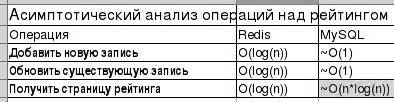
\includegraphics[width=10cm]{19_big_o_small.jpeg}

Как видим, серьёзной проблемой MySQL является очень дорогое получение страницы рейтинга.

Результат запуска бенчмарков отражен в сводной таблице:

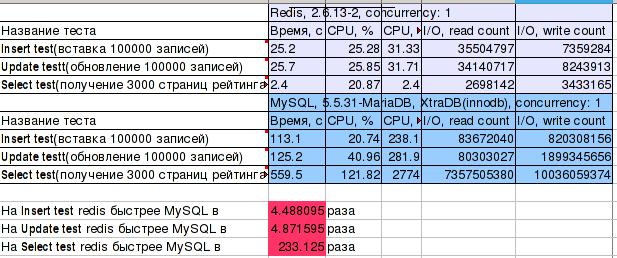
\includegraphics[width=10cm]{19_table_small.jpeg}

Как видно из таблицы, Redis значительно превосходит MySQL по производительности. На операциях вставки и обновления производительность выше почти в 5 раз, на операциях выборки превосходство просто подавляющее: 230 раз. При этом наличие необходимых индексов в MySQL таблице никак не влияет на производительность теста.

Несмотря на впечатляющие цифры на данном тесте, при анализе пригодности Redis к реализации других подзадач был выявлен ряд недостатков Redis: невозможность мультисортировки, избыточность данных при реализации рейтингов по уровню, проблемы с построением рейтинга среди друзей. Поэтому при решении задач построения различных игровых рейтингов оптимальным решением является использование этих двух СУБД в одной связке.

\end{document}
